\documentclass[11pt]{article}
\usepackage[textwidth=18.0cm, textheight=23.0cm, top=2.0cm]{geometry}
\usepackage{pst-all}
\usepackage{amssymb}
\usepackage{tikz}
\usepackage{underscore}\begin{document}
\pagestyle{empty}


ClassName: \underline{\textbf{Class_03.2bp-33}}
\par
BinSize: \underline{\textbf{40 × 40}}
\par
ReduceSize: \underline{\textbf{40 × 40}}
\par
TypeNum: \underline{\textbf{78}}
\par
Num: \underline{\textbf{80}}
\par
OutS: \underline{\textbf{28800}}
\par
InS: \underline{\textbf{26128}}
\par
Rate: \underline{\textbf{0.907}}
\par
UB: \underline{\textbf{18}}
\par
LB0: \underline{\textbf{18}}
\par
LB: \underline{\textbf{18}}
\par
LBWithCut: \underline{\textbf{18}}
\par
NodeCut: \underline{\textbf{0}}
\par
ExtendedNodeCnt: \underline{\textbf{1}}
\par
GenNodeCnt: \underline{\textbf{1}}
\par
PrimalNode: \underline{\textbf{0}}
\par
ColumnCount: \underline{\textbf{18}}
\par
TotalCutCount: \underline{\textbf{0}}
\par
RootCutCount: \underline{\textbf{0}}
\par
LPSolverCnt: \underline{\textbf{1}}
\par
PricingSolverCnt: \underline{\textbf{0}}
\par
BranchAndBoundNum: \underline{\textbf{1}}
\par
isOpt: \underline{\textbf{true}}
\par
TimeOnInitSolution: \underline{\textbf{600.000 s}}
\par
TimeOnPrimal: \underline{\textbf{0.000 s}}
\par
TimeOnPricing: \underline{\textbf{0.000 s}}
\par
TimeOnRmp: \underline{\textbf{0.062 s}}
\par
TotalTime: \underline{\textbf{600.328 s}}
\par
\newpage


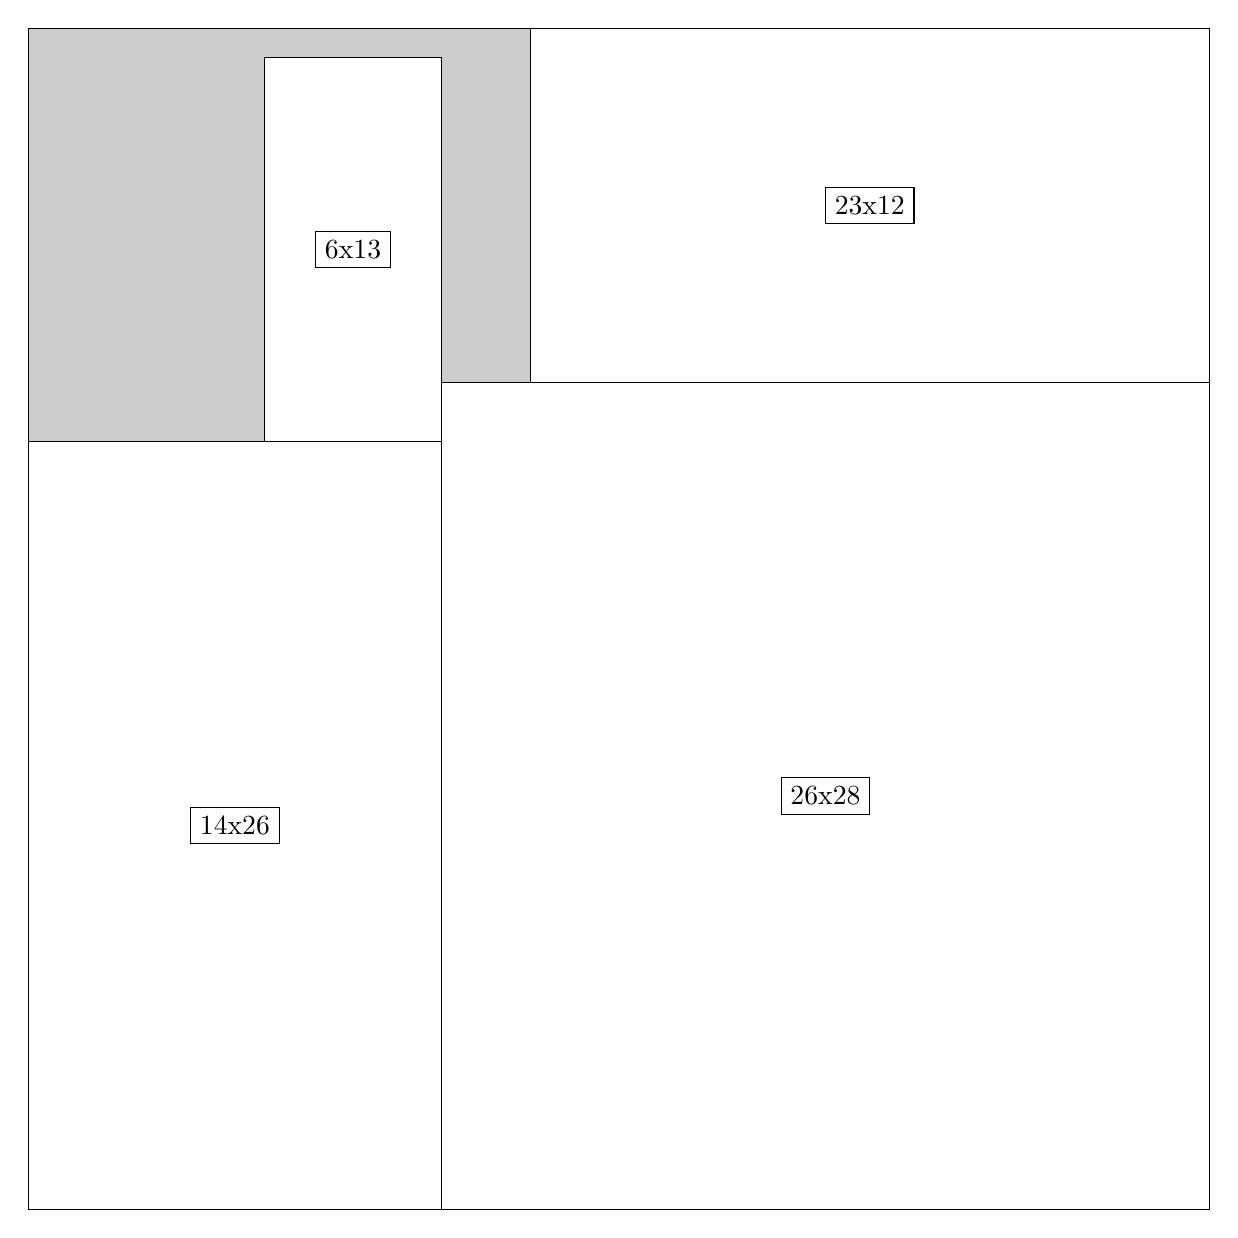
\begin{tikzpicture}[shorten >=1pt,scale=1.0,every node/.style={scale=1.0},->]
\tikzstyle{vertex}=[circle,fill=black!25,minimum size=14pt,inner sep=0pt]
\filldraw[fill=gray!40!white, draw=black] (0,0) rectangle (15.0,15.0);
\foreach \name/\x/\y/\w/\h in {26x28/5.25/0.0/9.75/10.5,23x12/6.375/10.5/8.625/4.5,14x26/0.0/0.0/5.25/9.75,6x13/3.0/9.75/2.25/4.875}
\filldraw[fill=white!40!white, draw=black] (\x,\y) rectangle node[draw] (\name) {\name} ++(\w,\h);
\end{tikzpicture}


w =26 , h =28 , x =14 , y =0 , v =728
\par
w =23 , h =12 , x =17 , y =28 , v =276
\par
w =14 , h =26 , x =0 , y =0 , v =364
\par
w =6 , h =13 , x =8 , y =26 , v =78
\par
\newpage


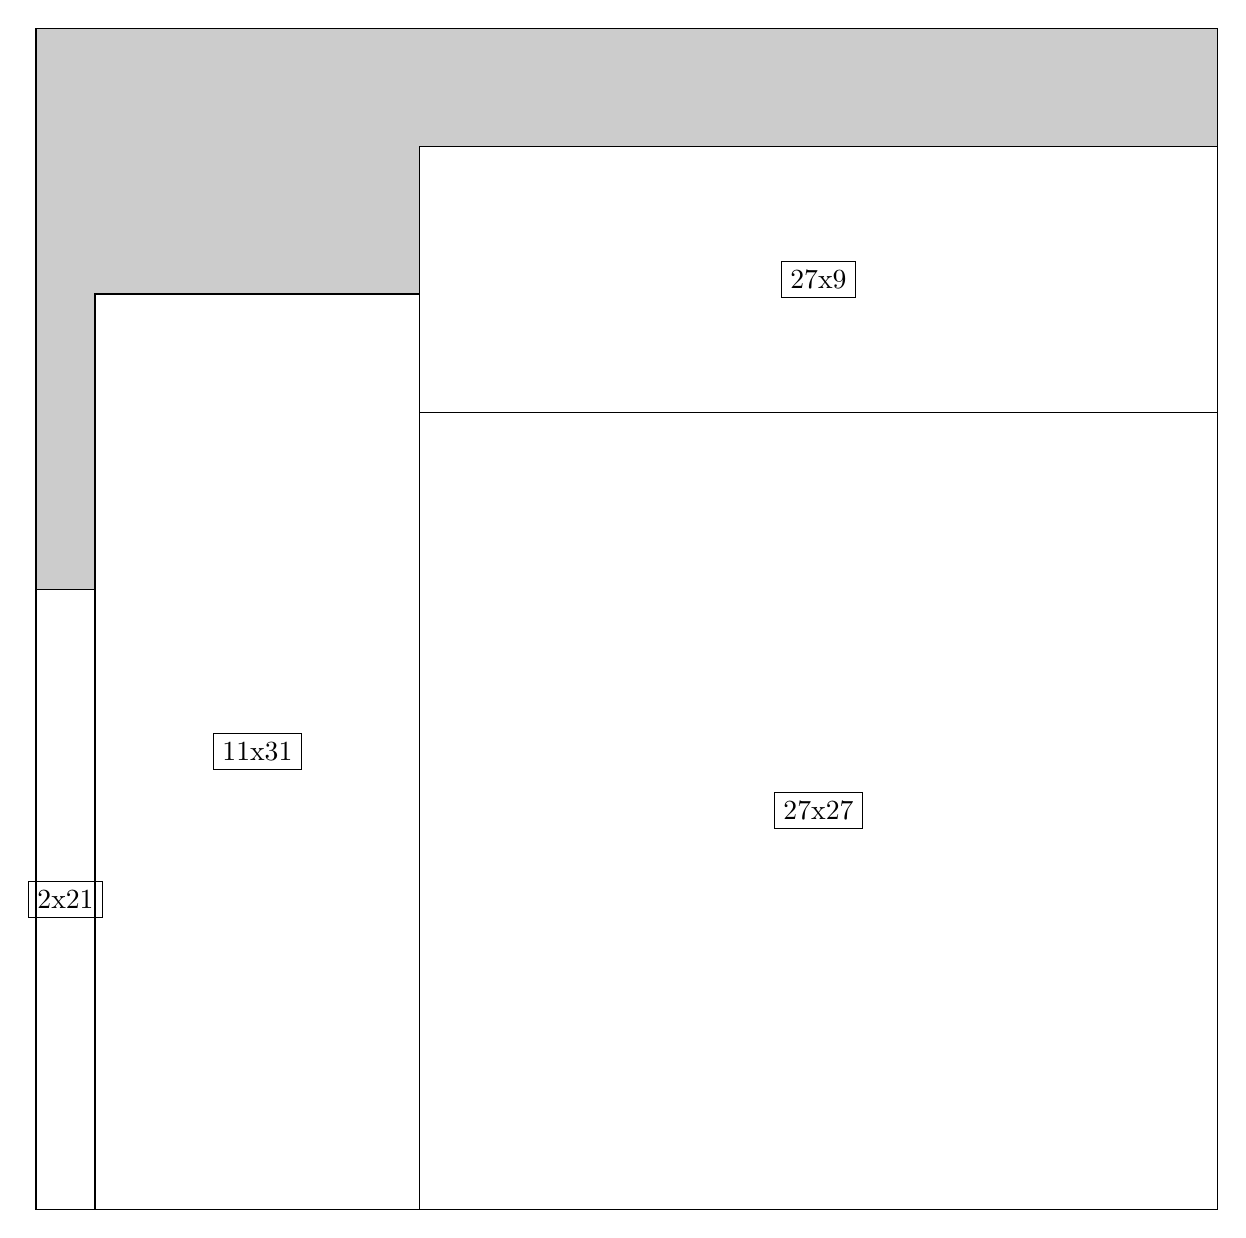
\begin{tikzpicture}[shorten >=1pt,scale=1.0,every node/.style={scale=1.0},->]
\tikzstyle{vertex}=[circle,fill=black!25,minimum size=14pt,inner sep=0pt]
\filldraw[fill=gray!40!white, draw=black] (0,0) rectangle (15.0,15.0);
\foreach \name/\x/\y/\w/\h in {27x27/4.875/0.0/10.125/10.125,27x9/4.875/10.125/10.125/3.375,11x31/0.75/0.0/4.125/11.625,2x21/0.0/0.0/0.75/7.875}
\filldraw[fill=white!40!white, draw=black] (\x,\y) rectangle node[draw] (\name) {\name} ++(\w,\h);
\end{tikzpicture}


w =27 , h =27 , x =13 , y =0 , v =729
\par
w =27 , h =9 , x =13 , y =27 , v =243
\par
w =11 , h =31 , x =2 , y =0 , v =341
\par
w =2 , h =21 , x =0 , y =0 , v =42
\par
\newpage


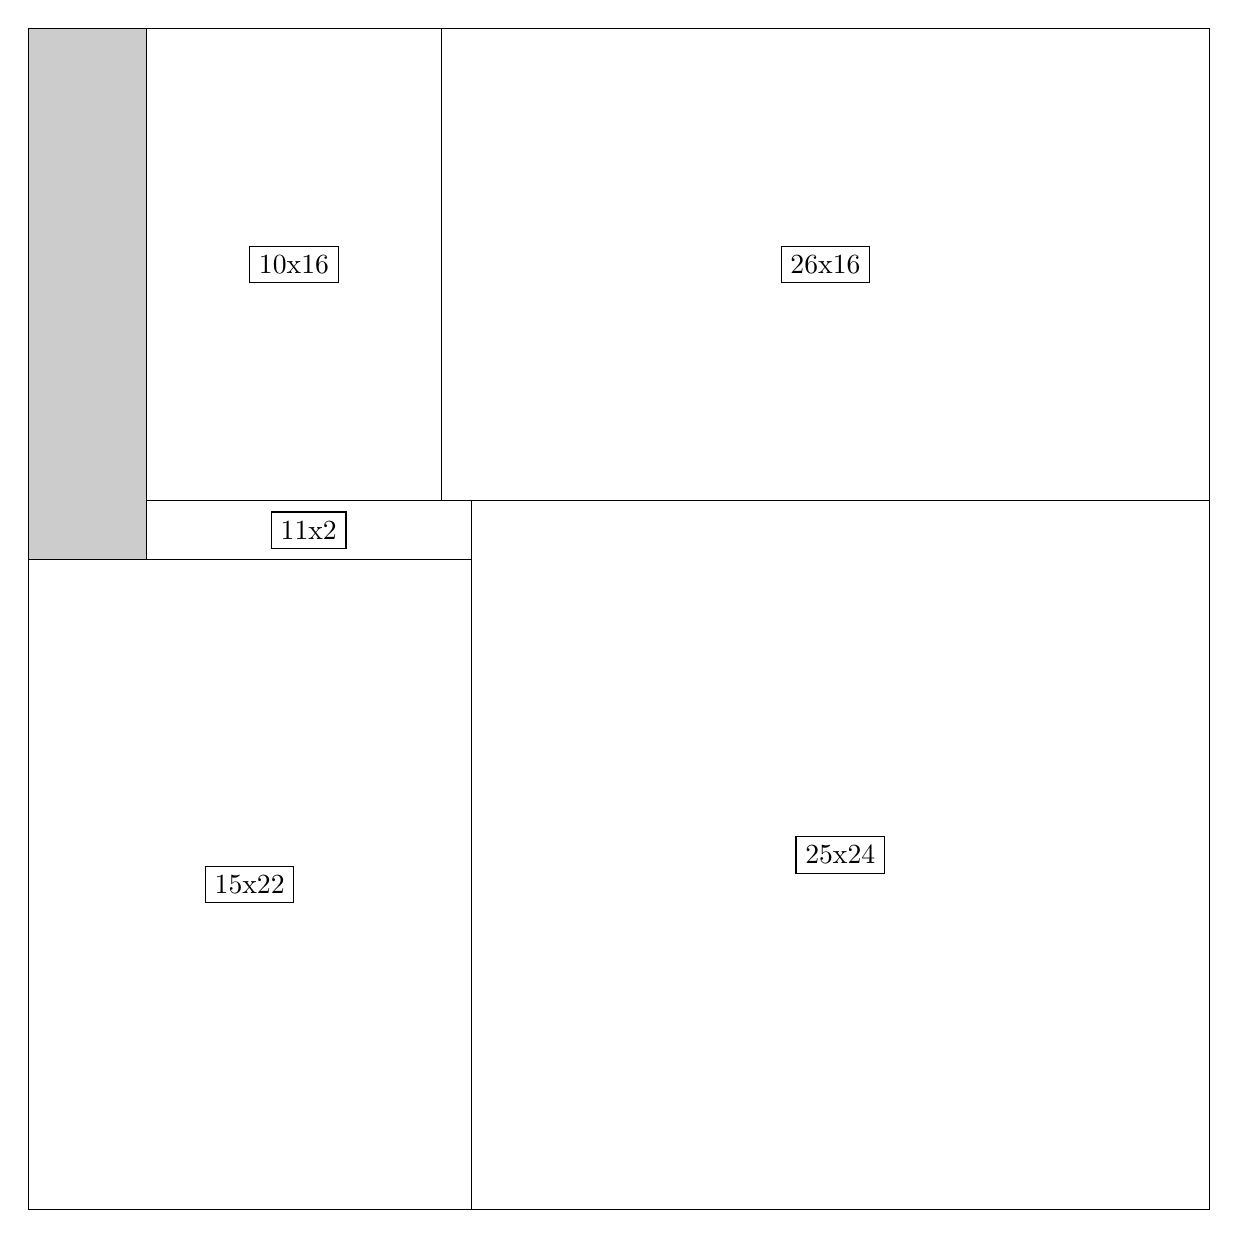
\begin{tikzpicture}[shorten >=1pt,scale=1.0,every node/.style={scale=1.0},->]
\tikzstyle{vertex}=[circle,fill=black!25,minimum size=14pt,inner sep=0pt]
\filldraw[fill=gray!40!white, draw=black] (0,0) rectangle (15.0,15.0);
\foreach \name/\x/\y/\w/\h in {25x24/5.625/0.0/9.375/9.0,15x22/0.0/0.0/5.625/8.25,11x2/1.5/8.25/4.125/0.75,26x16/5.25/9.0/9.75/6.0,10x16/1.5/9.0/3.75/6.0}
\filldraw[fill=white!40!white, draw=black] (\x,\y) rectangle node[draw] (\name) {\name} ++(\w,\h);
\end{tikzpicture}


w =25 , h =24 , x =15 , y =0 , v =600
\par
w =15 , h =22 , x =0 , y =0 , v =330
\par
w =11 , h =2 , x =4 , y =22 , v =22
\par
w =26 , h =16 , x =14 , y =24 , v =416
\par
w =10 , h =16 , x =4 , y =24 , v =160
\par
\newpage


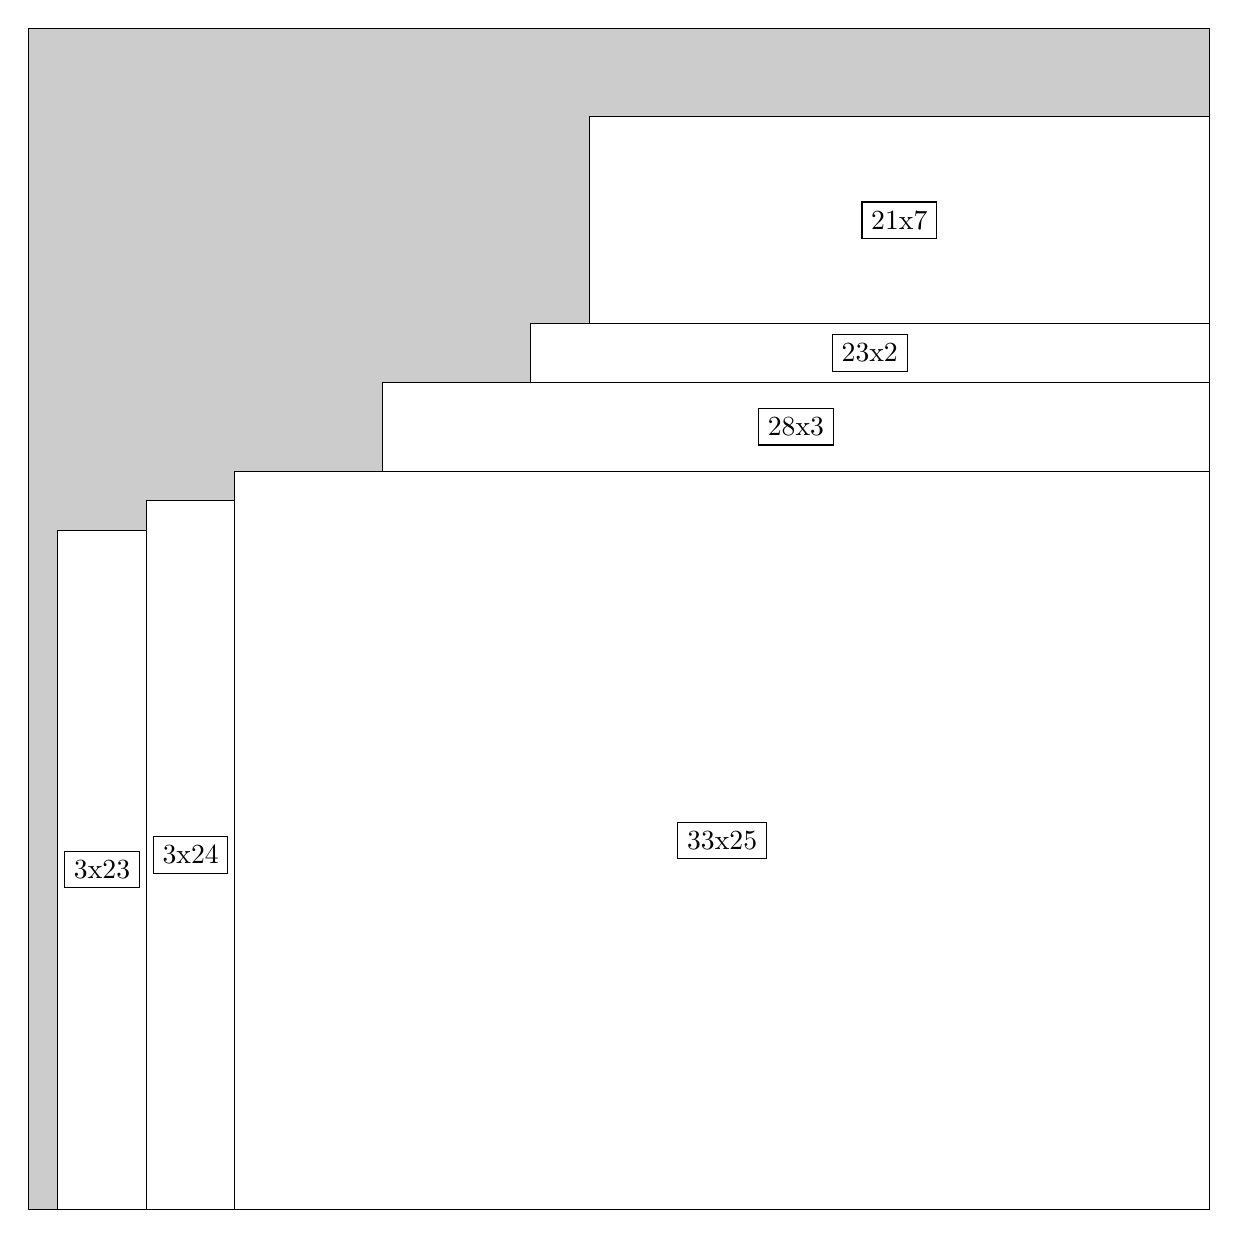
\begin{tikzpicture}[shorten >=1pt,scale=1.0,every node/.style={scale=1.0},->]
\tikzstyle{vertex}=[circle,fill=black!25,minimum size=14pt,inner sep=0pt]
\filldraw[fill=gray!40!white, draw=black] (0,0) rectangle (15.0,15.0);
\foreach \name/\x/\y/\w/\h in {33x25/2.625/0.0/12.375/9.375,3x24/1.5/0.0/1.125/9.0,3x23/0.375/0.0/1.125/8.625,28x3/4.5/9.375/10.5/1.125,23x2/6.375/10.5/8.625/0.75,21x7/7.125/11.25/7.875/2.625}
\filldraw[fill=white!40!white, draw=black] (\x,\y) rectangle node[draw] (\name) {\name} ++(\w,\h);
\end{tikzpicture}


w =33 , h =25 , x =7 , y =0 , v =825
\par
w =3 , h =24 , x =4 , y =0 , v =72
\par
w =3 , h =23 , x =1 , y =0 , v =69
\par
w =28 , h =3 , x =12 , y =25 , v =84
\par
w =23 , h =2 , x =17 , y =28 , v =46
\par
w =21 , h =7 , x =19 , y =30 , v =147
\par
\newpage


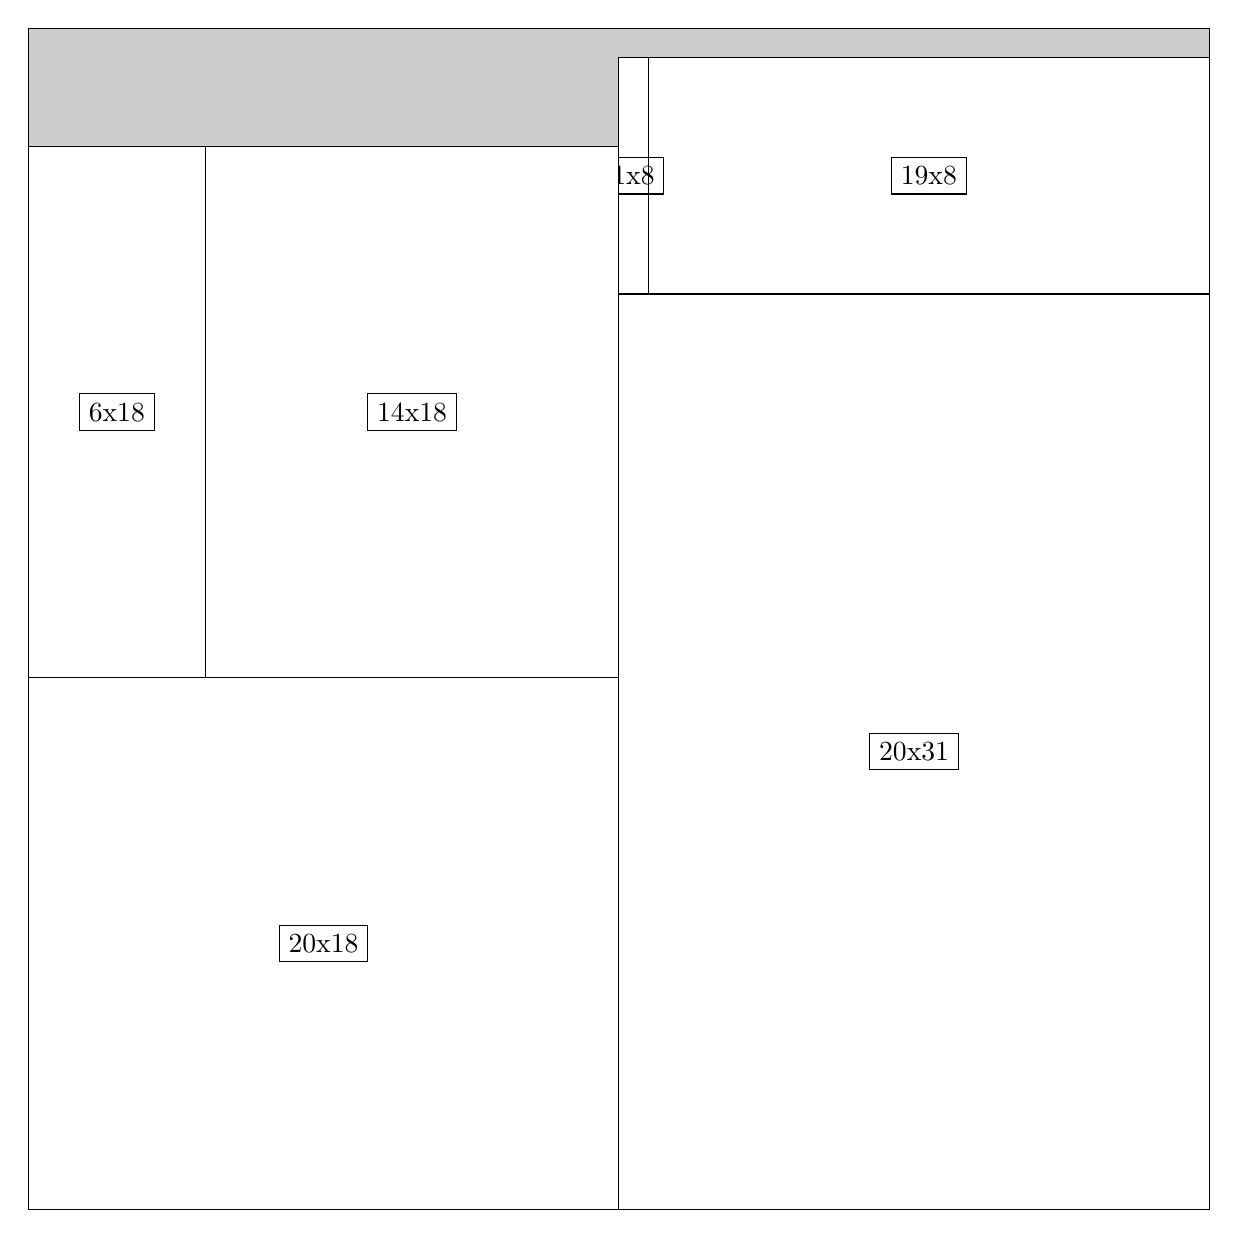
\begin{tikzpicture}[shorten >=1pt,scale=1.0,every node/.style={scale=1.0},->]
\tikzstyle{vertex}=[circle,fill=black!25,minimum size=14pt,inner sep=0pt]
\filldraw[fill=gray!40!white, draw=black] (0,0) rectangle (15.0,15.0);
\foreach \name/\x/\y/\w/\h in {20x31/7.5/0.0/7.5/11.625,19x8/7.875/11.625/7.125/3.0,1x8/7.5/11.625/0.375/3.0,20x18/0.0/0.0/7.5/6.75,14x18/2.25/6.75/5.25/6.75,6x18/0.0/6.75/2.25/6.75}
\filldraw[fill=white!40!white, draw=black] (\x,\y) rectangle node[draw] (\name) {\name} ++(\w,\h);
\end{tikzpicture}


w =20 , h =31 , x =20 , y =0 , v =620
\par
w =19 , h =8 , x =21 , y =31 , v =152
\par
w =1 , h =8 , x =20 , y =31 , v =8
\par
w =20 , h =18 , x =0 , y =0 , v =360
\par
w =14 , h =18 , x =6 , y =18 , v =252
\par
w =6 , h =18 , x =0 , y =18 , v =108
\par
\newpage


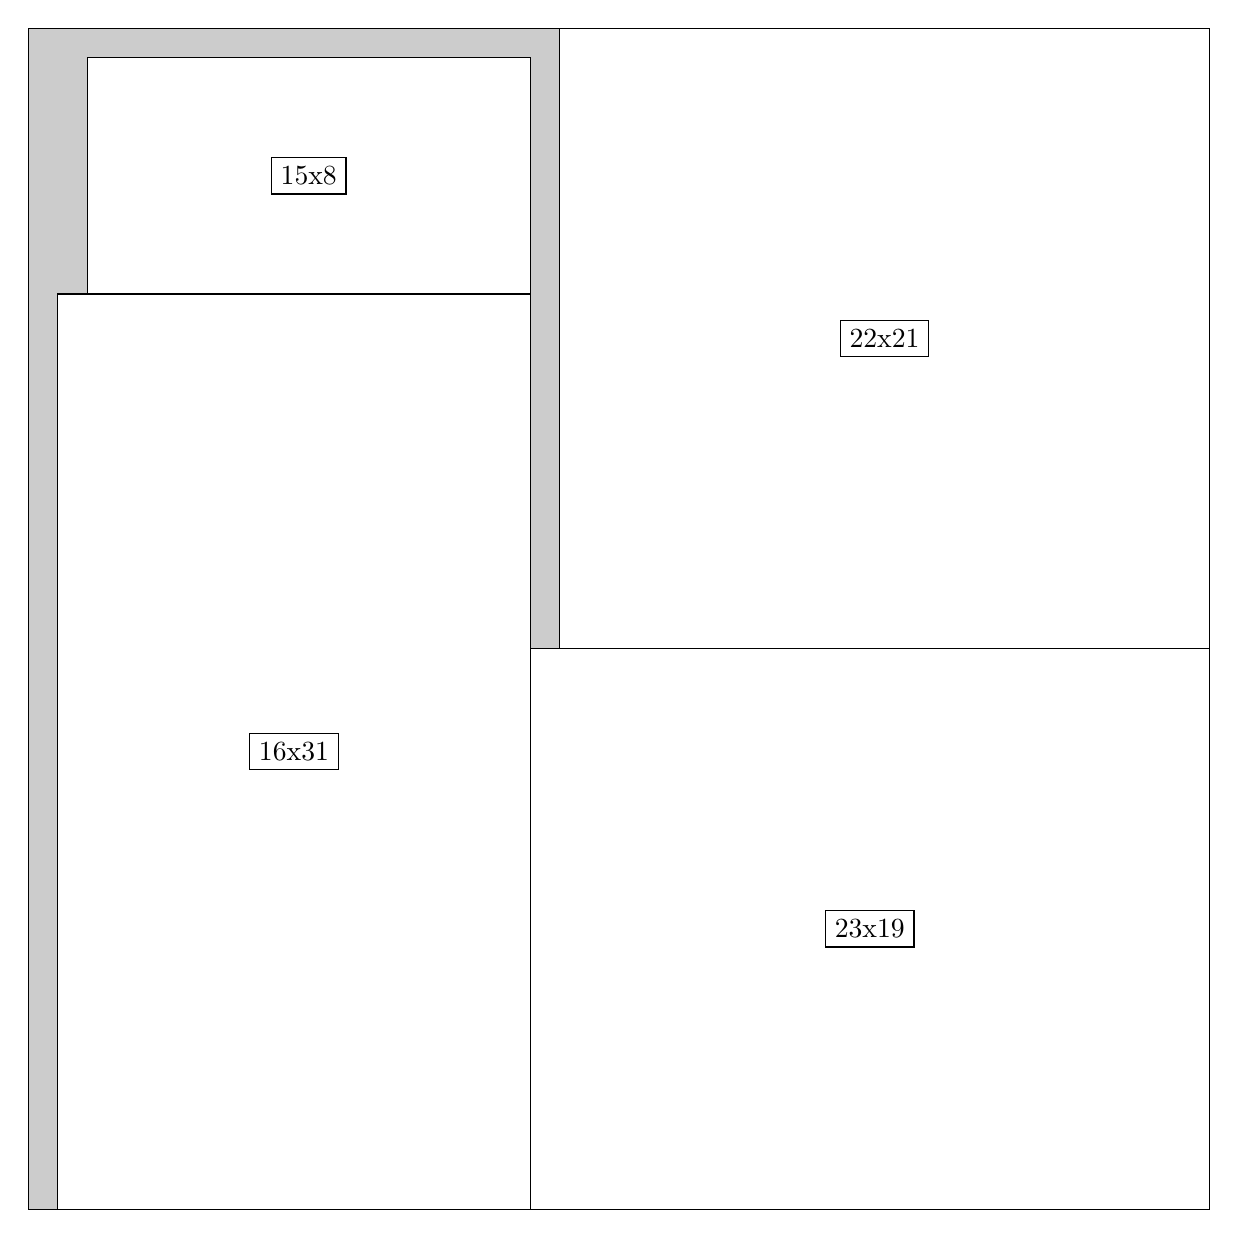
\begin{tikzpicture}[shorten >=1pt,scale=1.0,every node/.style={scale=1.0},->]
\tikzstyle{vertex}=[circle,fill=black!25,minimum size=14pt,inner sep=0pt]
\filldraw[fill=gray!40!white, draw=black] (0,0) rectangle (15.0,15.0);
\foreach \name/\x/\y/\w/\h in {23x19/6.375/0.0/8.625/7.125,22x21/6.75/7.125/8.25/7.875,16x31/0.375/0.0/6.0/11.625,15x8/0.75/11.625/5.625/3.0}
\filldraw[fill=white!40!white, draw=black] (\x,\y) rectangle node[draw] (\name) {\name} ++(\w,\h);
\end{tikzpicture}


w =23 , h =19 , x =17 , y =0 , v =437
\par
w =22 , h =21 , x =18 , y =19 , v =462
\par
w =16 , h =31 , x =1 , y =0 , v =496
\par
w =15 , h =8 , x =2 , y =31 , v =120
\par
\newpage


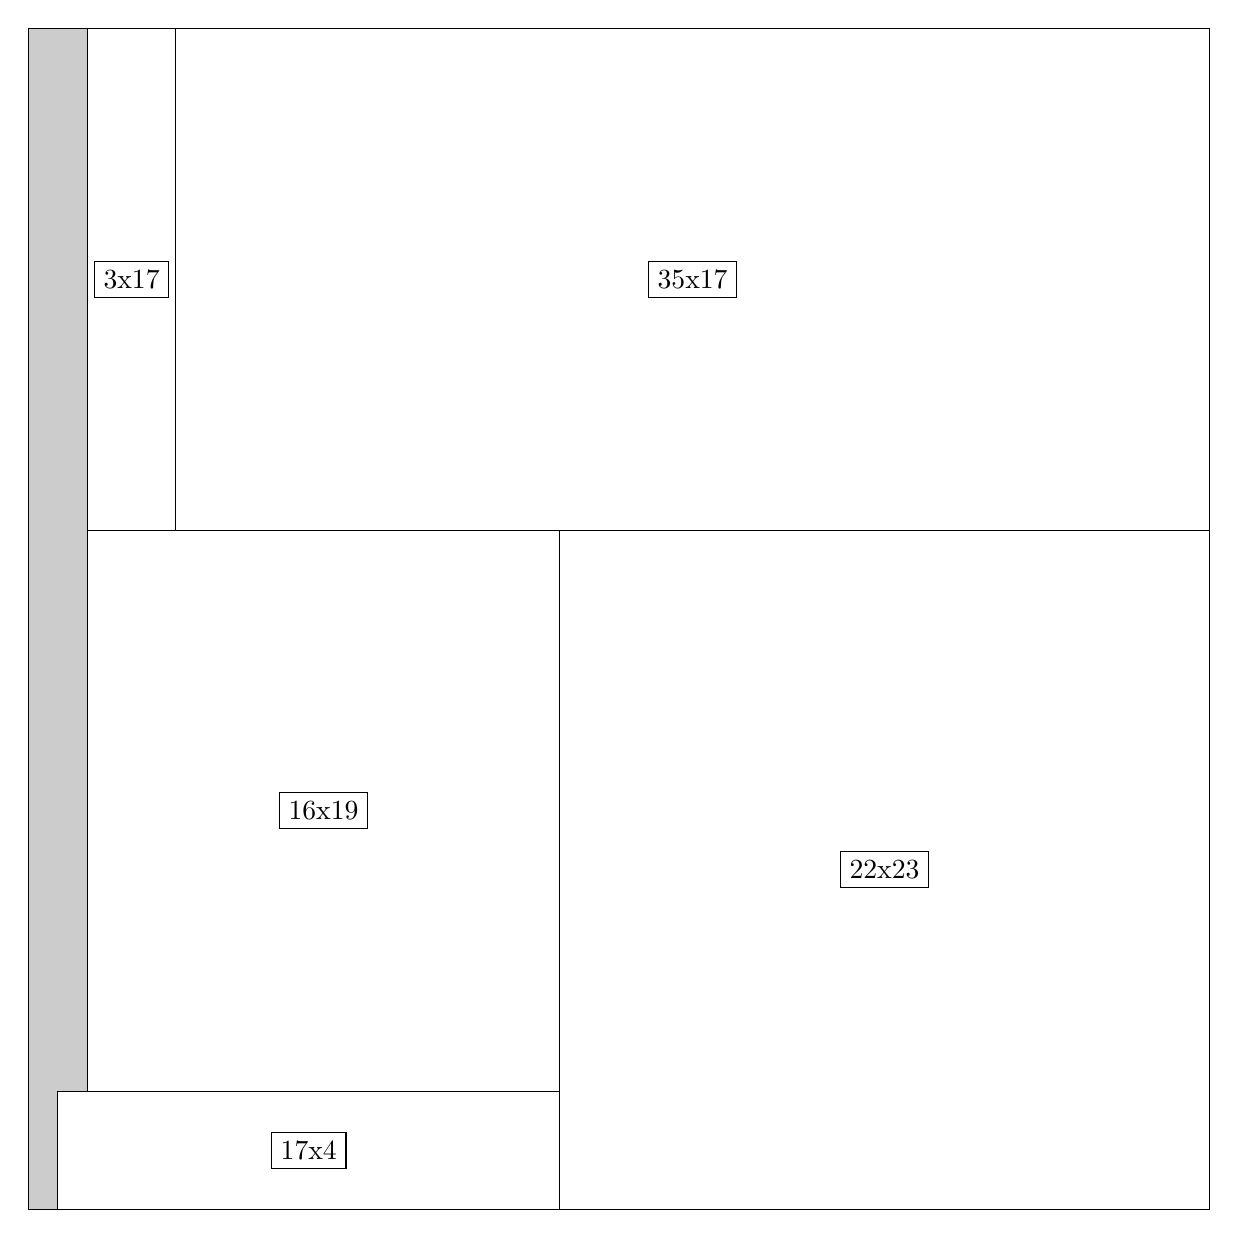
\begin{tikzpicture}[shorten >=1pt,scale=1.0,every node/.style={scale=1.0},->]
\tikzstyle{vertex}=[circle,fill=black!25,minimum size=14pt,inner sep=0pt]
\filldraw[fill=gray!40!white, draw=black] (0,0) rectangle (15.0,15.0);
\foreach \name/\x/\y/\w/\h in {22x23/6.75/0.0/8.25/8.625,17x4/0.375/0.0/6.375/1.5,16x19/0.75/1.5/6.0/7.125,35x17/1.875/8.625/13.125/6.375,3x17/0.75/8.625/1.125/6.375}
\filldraw[fill=white!40!white, draw=black] (\x,\y) rectangle node[draw] (\name) {\name} ++(\w,\h);
\end{tikzpicture}


w =22 , h =23 , x =18 , y =0 , v =506
\par
w =17 , h =4 , x =1 , y =0 , v =68
\par
w =16 , h =19 , x =2 , y =4 , v =304
\par
w =35 , h =17 , x =5 , y =23 , v =595
\par
w =3 , h =17 , x =2 , y =23 , v =51
\par
\newpage


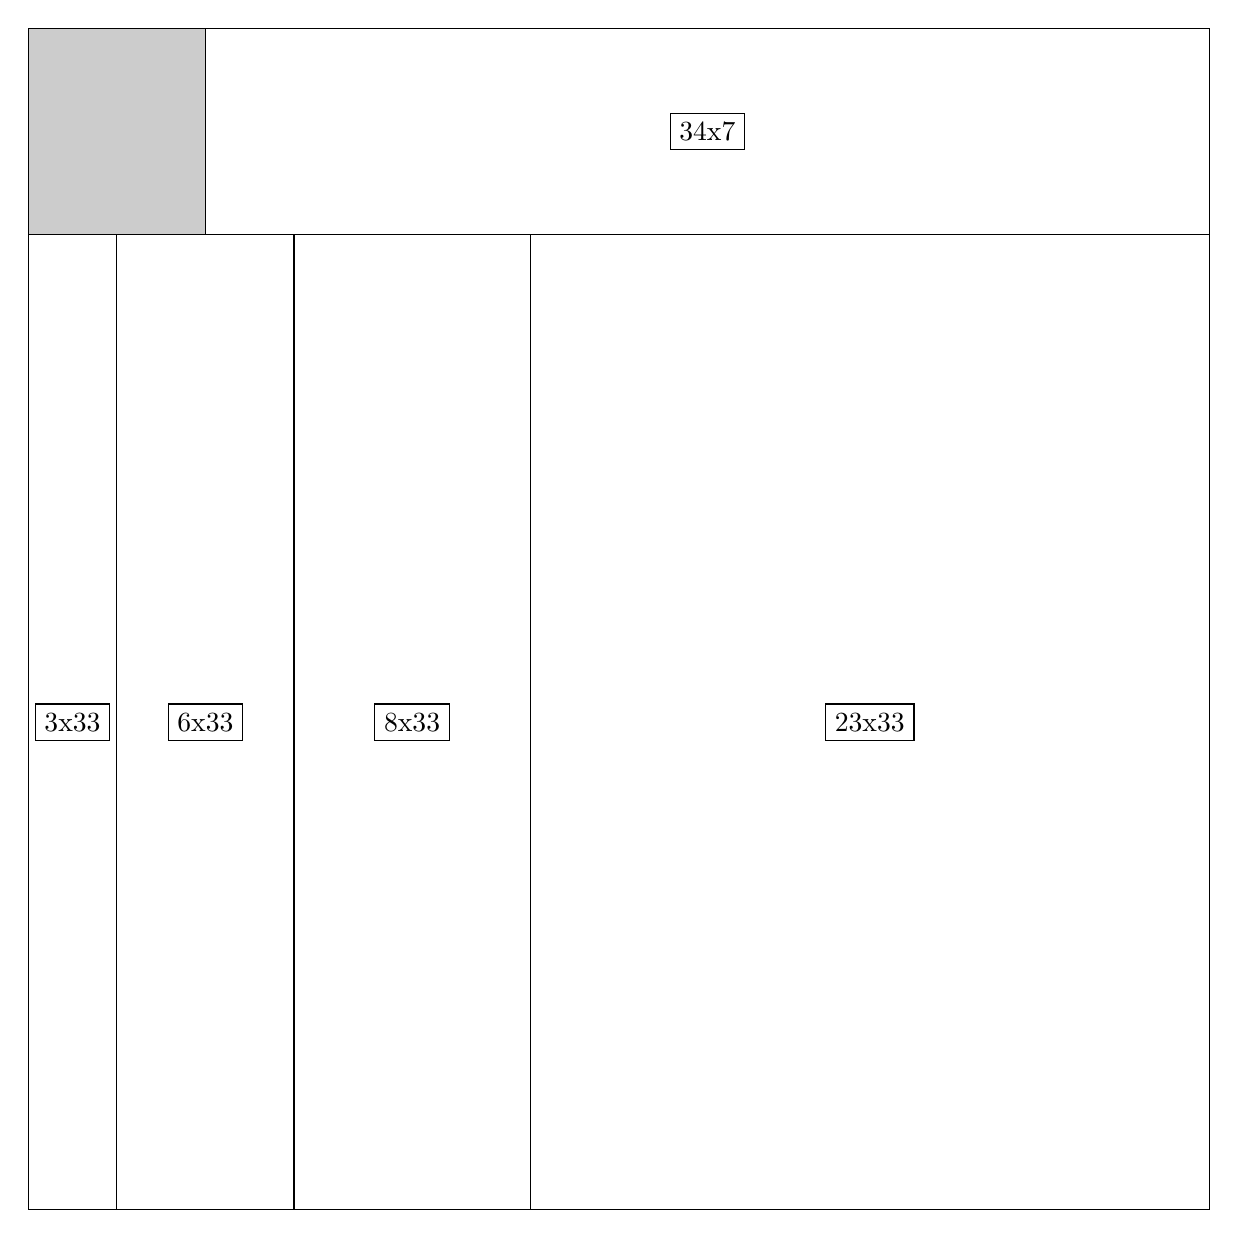
\begin{tikzpicture}[shorten >=1pt,scale=1.0,every node/.style={scale=1.0},->]
\tikzstyle{vertex}=[circle,fill=black!25,minimum size=14pt,inner sep=0pt]
\filldraw[fill=gray!40!white, draw=black] (0,0) rectangle (15.0,15.0);
\foreach \name/\x/\y/\w/\h in {23x33/6.375/0.0/8.625/12.375,8x33/3.375/0.0/3.0/12.375,6x33/1.125/0.0/2.25/12.375,3x33/0.0/0.0/1.125/12.375,34x7/2.25/12.375/12.75/2.625}
\filldraw[fill=white!40!white, draw=black] (\x,\y) rectangle node[draw] (\name) {\name} ++(\w,\h);
\end{tikzpicture}


w =23 , h =33 , x =17 , y =0 , v =759
\par
w =8 , h =33 , x =9 , y =0 , v =264
\par
w =6 , h =33 , x =3 , y =0 , v =198
\par
w =3 , h =33 , x =0 , y =0 , v =99
\par
w =34 , h =7 , x =6 , y =33 , v =238
\par
\newpage


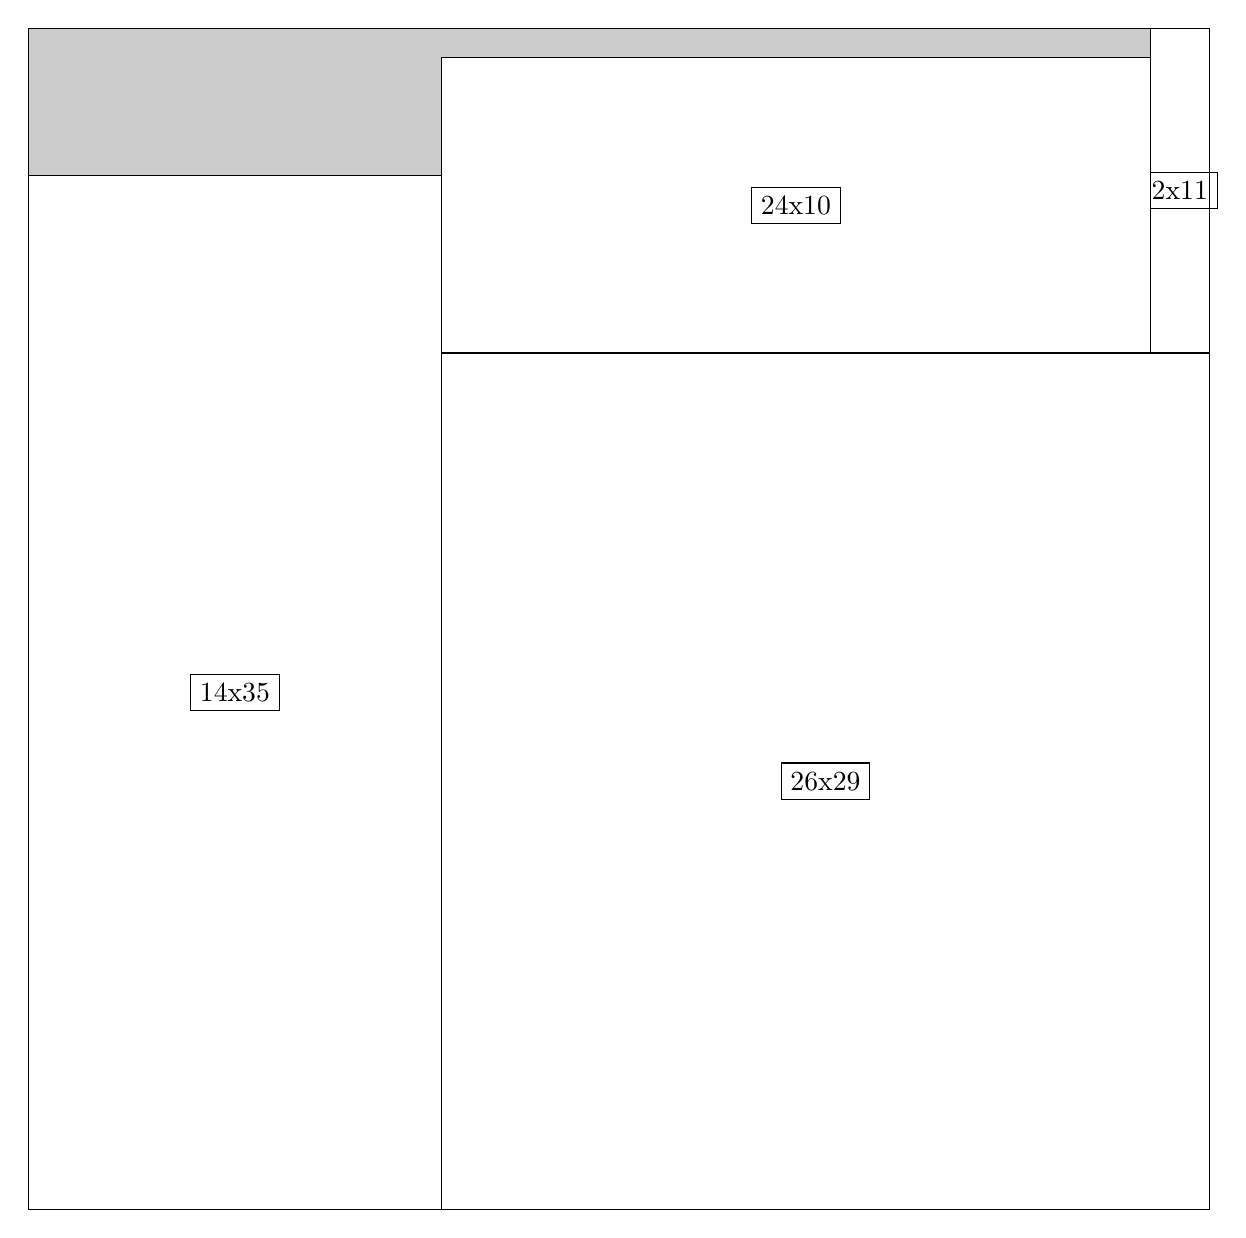
\begin{tikzpicture}[shorten >=1pt,scale=1.0,every node/.style={scale=1.0},->]
\tikzstyle{vertex}=[circle,fill=black!25,minimum size=14pt,inner sep=0pt]
\filldraw[fill=gray!40!white, draw=black] (0,0) rectangle (15.0,15.0);
\foreach \name/\x/\y/\w/\h in {26x29/5.25/0.0/9.75/10.875,2x11/14.25/10.875/0.75/4.125,24x10/5.25/10.875/9.0/3.75,14x35/0.0/0.0/5.25/13.125}
\filldraw[fill=white!40!white, draw=black] (\x,\y) rectangle node[draw] (\name) {\name} ++(\w,\h);
\end{tikzpicture}


w =26 , h =29 , x =14 , y =0 , v =754
\par
w =2 , h =11 , x =38 , y =29 , v =22
\par
w =24 , h =10 , x =14 , y =29 , v =240
\par
w =14 , h =35 , x =0 , y =0 , v =490
\par
\newpage


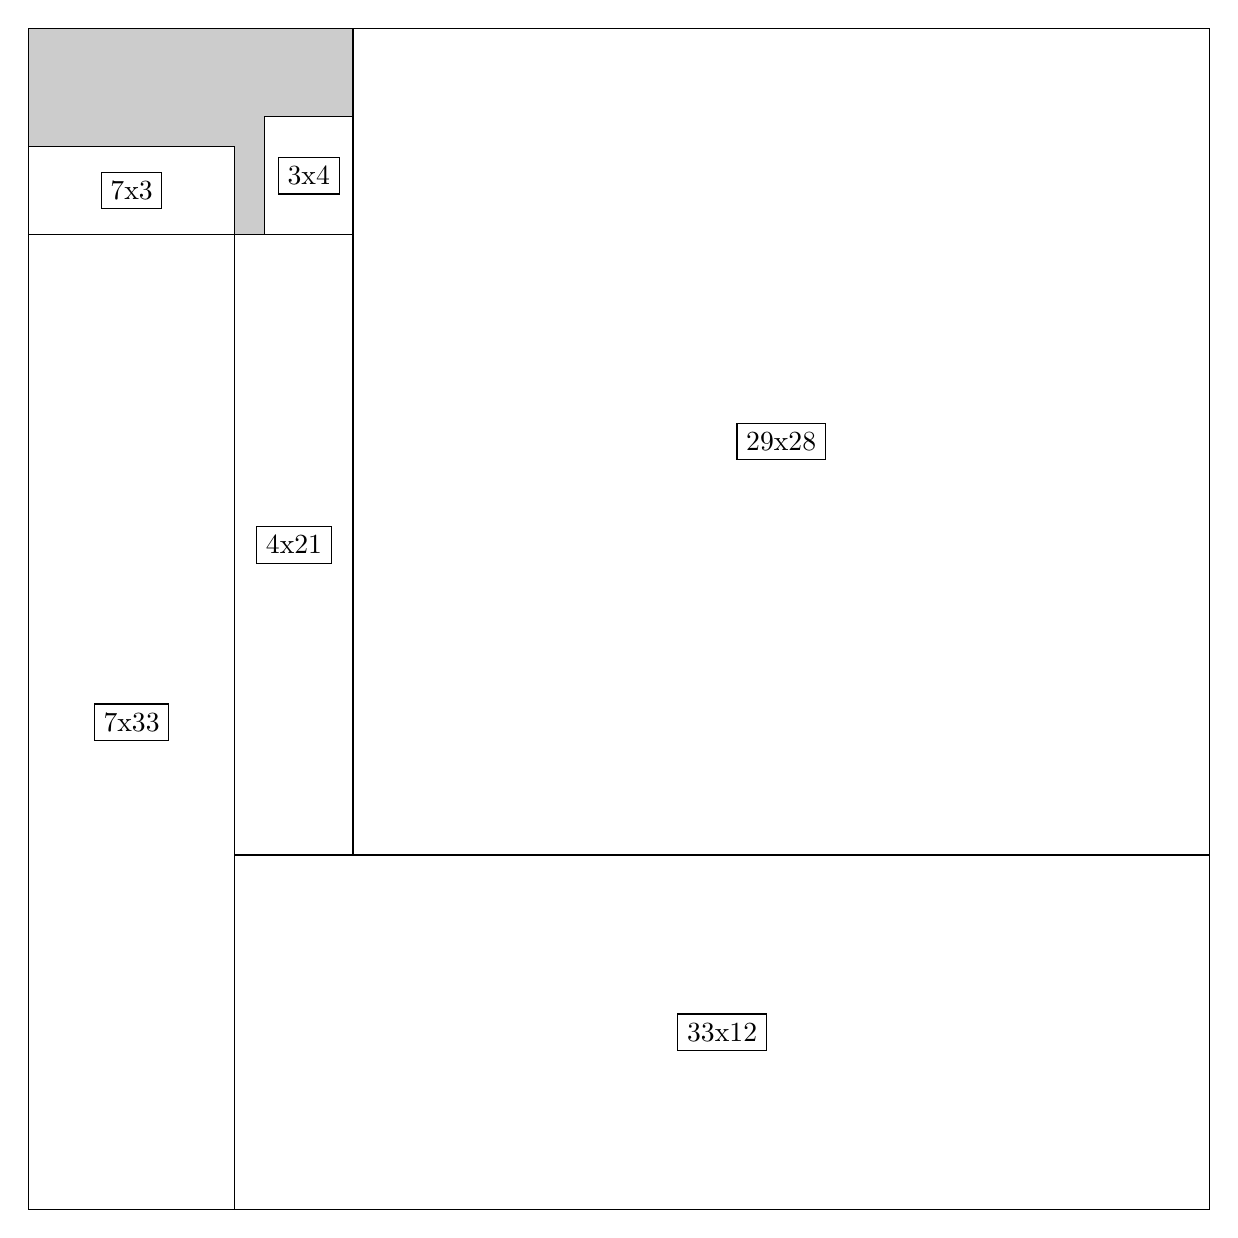
\begin{tikzpicture}[shorten >=1pt,scale=1.0,every node/.style={scale=1.0},->]
\tikzstyle{vertex}=[circle,fill=black!25,minimum size=14pt,inner sep=0pt]
\filldraw[fill=gray!40!white, draw=black] (0,0) rectangle (15.0,15.0);
\foreach \name/\x/\y/\w/\h in {33x12/2.625/0.0/12.375/4.5,29x28/4.125/4.5/10.875/10.5,4x21/2.625/4.5/1.5/7.875,3x4/3.0/12.375/1.125/1.5,7x33/0.0/0.0/2.625/12.375,7x3/0.0/12.375/2.625/1.125}
\filldraw[fill=white!40!white, draw=black] (\x,\y) rectangle node[draw] (\name) {\name} ++(\w,\h);
\end{tikzpicture}


w =33 , h =12 , x =7 , y =0 , v =396
\par
w =29 , h =28 , x =11 , y =12 , v =812
\par
w =4 , h =21 , x =7 , y =12 , v =84
\par
w =3 , h =4 , x =8 , y =33 , v =12
\par
w =7 , h =33 , x =0 , y =0 , v =231
\par
w =7 , h =3 , x =0 , y =33 , v =21
\par
\newpage


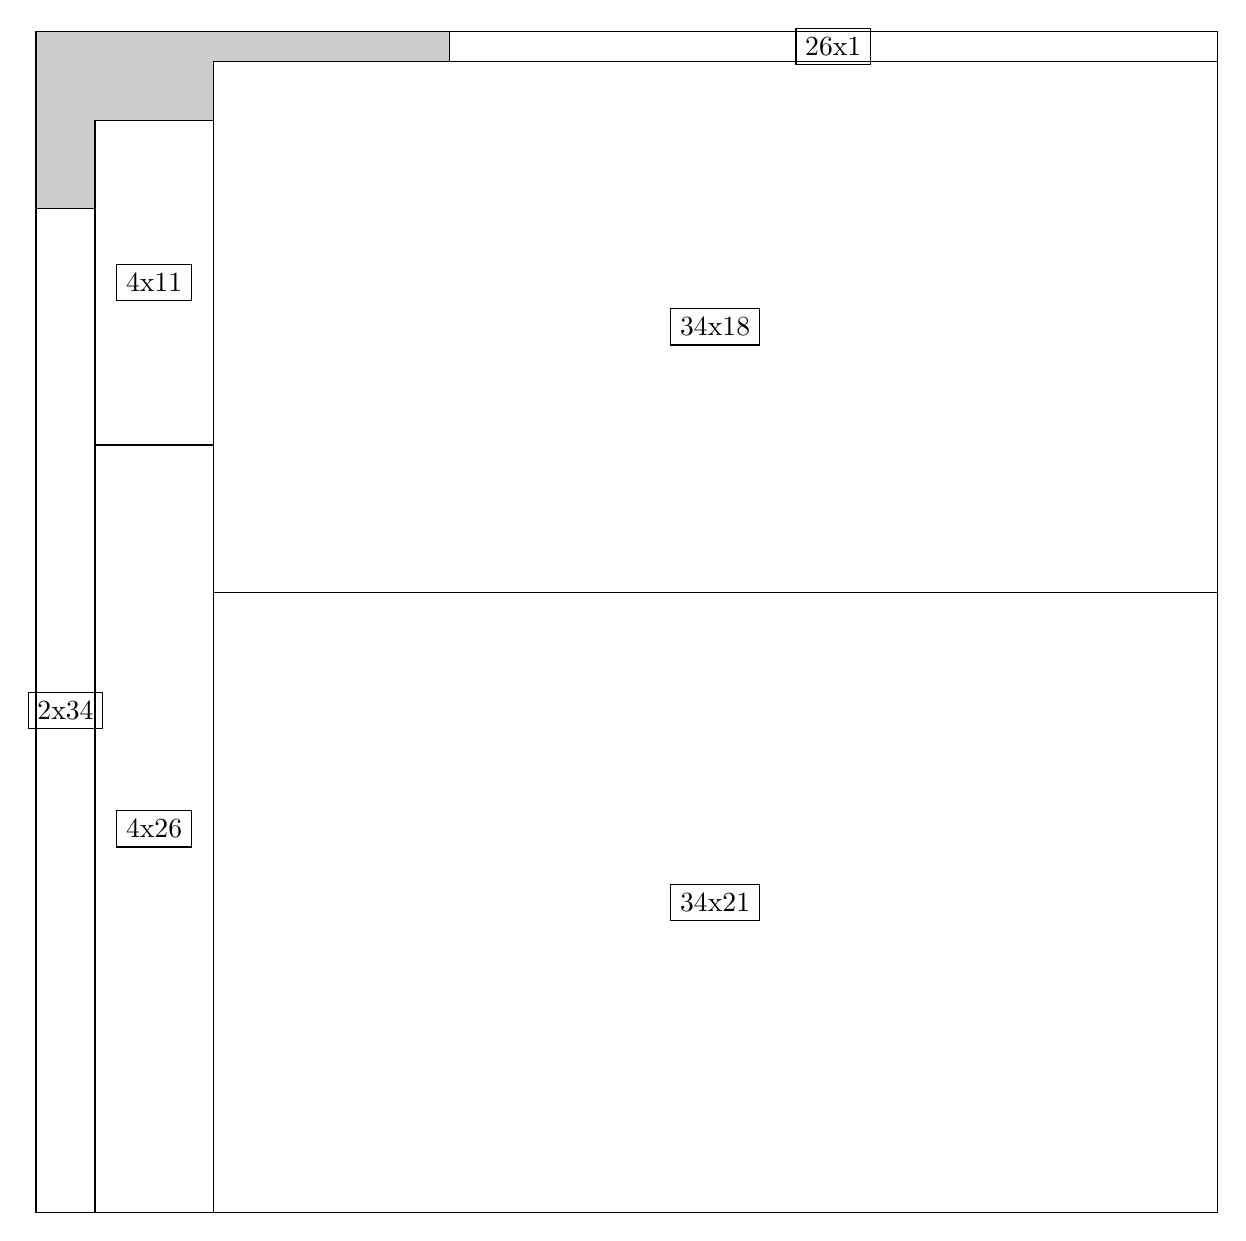
\begin{tikzpicture}[shorten >=1pt,scale=1.0,every node/.style={scale=1.0},->]
\tikzstyle{vertex}=[circle,fill=black!25,minimum size=14pt,inner sep=0pt]
\filldraw[fill=gray!40!white, draw=black] (0,0) rectangle (15.0,15.0);
\foreach \name/\x/\y/\w/\h in {34x21/2.25/0.0/12.75/7.875,34x18/2.25/7.875/12.75/6.75,26x1/5.25/14.625/9.75/0.375,4x26/0.75/0.0/1.5/9.75,4x11/0.75/9.75/1.5/4.125,2x34/0.0/0.0/0.75/12.75}
\filldraw[fill=white!40!white, draw=black] (\x,\y) rectangle node[draw] (\name) {\name} ++(\w,\h);
\end{tikzpicture}


w =34 , h =21 , x =6 , y =0 , v =714
\par
w =34 , h =18 , x =6 , y =21 , v =612
\par
w =26 , h =1 , x =14 , y =39 , v =26
\par
w =4 , h =26 , x =2 , y =0 , v =104
\par
w =4 , h =11 , x =2 , y =26 , v =44
\par
w =2 , h =34 , x =0 , y =0 , v =68
\par
\newpage


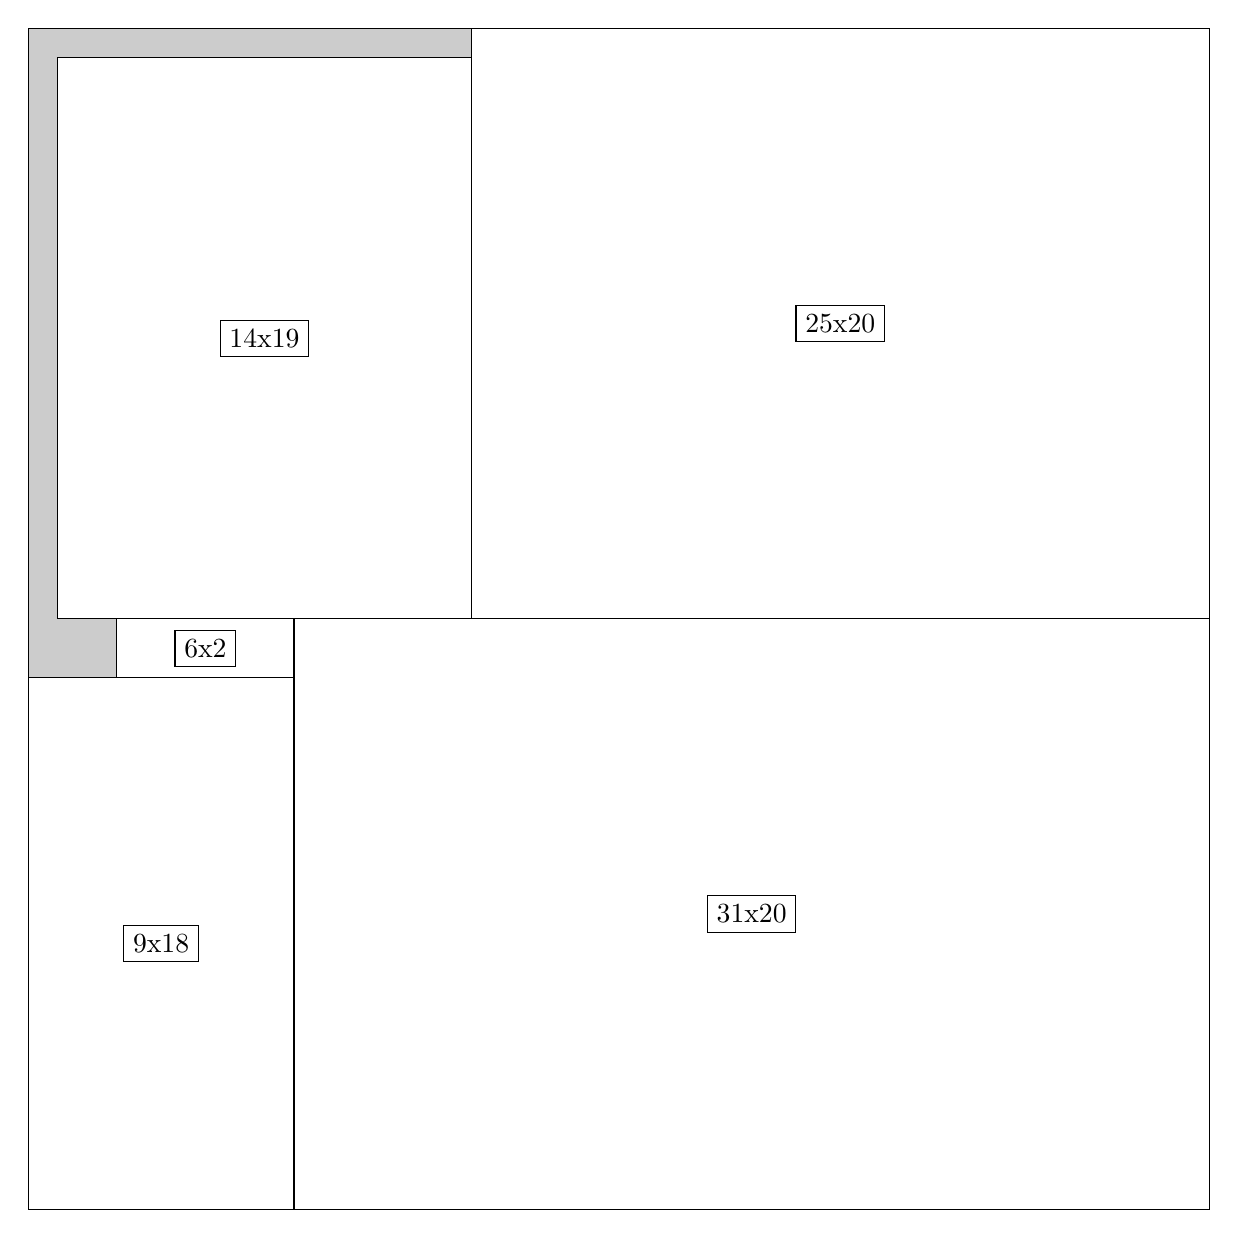
\begin{tikzpicture}[shorten >=1pt,scale=1.0,every node/.style={scale=1.0},->]
\tikzstyle{vertex}=[circle,fill=black!25,minimum size=14pt,inner sep=0pt]
\filldraw[fill=gray!40!white, draw=black] (0,0) rectangle (15.0,15.0);
\foreach \name/\x/\y/\w/\h in {31x20/3.375/0.0/11.625/7.5,9x18/0.0/0.0/3.375/6.75,6x2/1.125/6.75/2.25/0.75,25x20/5.625/7.5/9.375/7.5,14x19/0.375/7.5/5.25/7.125}
\filldraw[fill=white!40!white, draw=black] (\x,\y) rectangle node[draw] (\name) {\name} ++(\w,\h);
\end{tikzpicture}


w =31 , h =20 , x =9 , y =0 , v =620
\par
w =9 , h =18 , x =0 , y =0 , v =162
\par
w =6 , h =2 , x =3 , y =18 , v =12
\par
w =25 , h =20 , x =15 , y =20 , v =500
\par
w =14 , h =19 , x =1 , y =20 , v =266
\par
\newpage


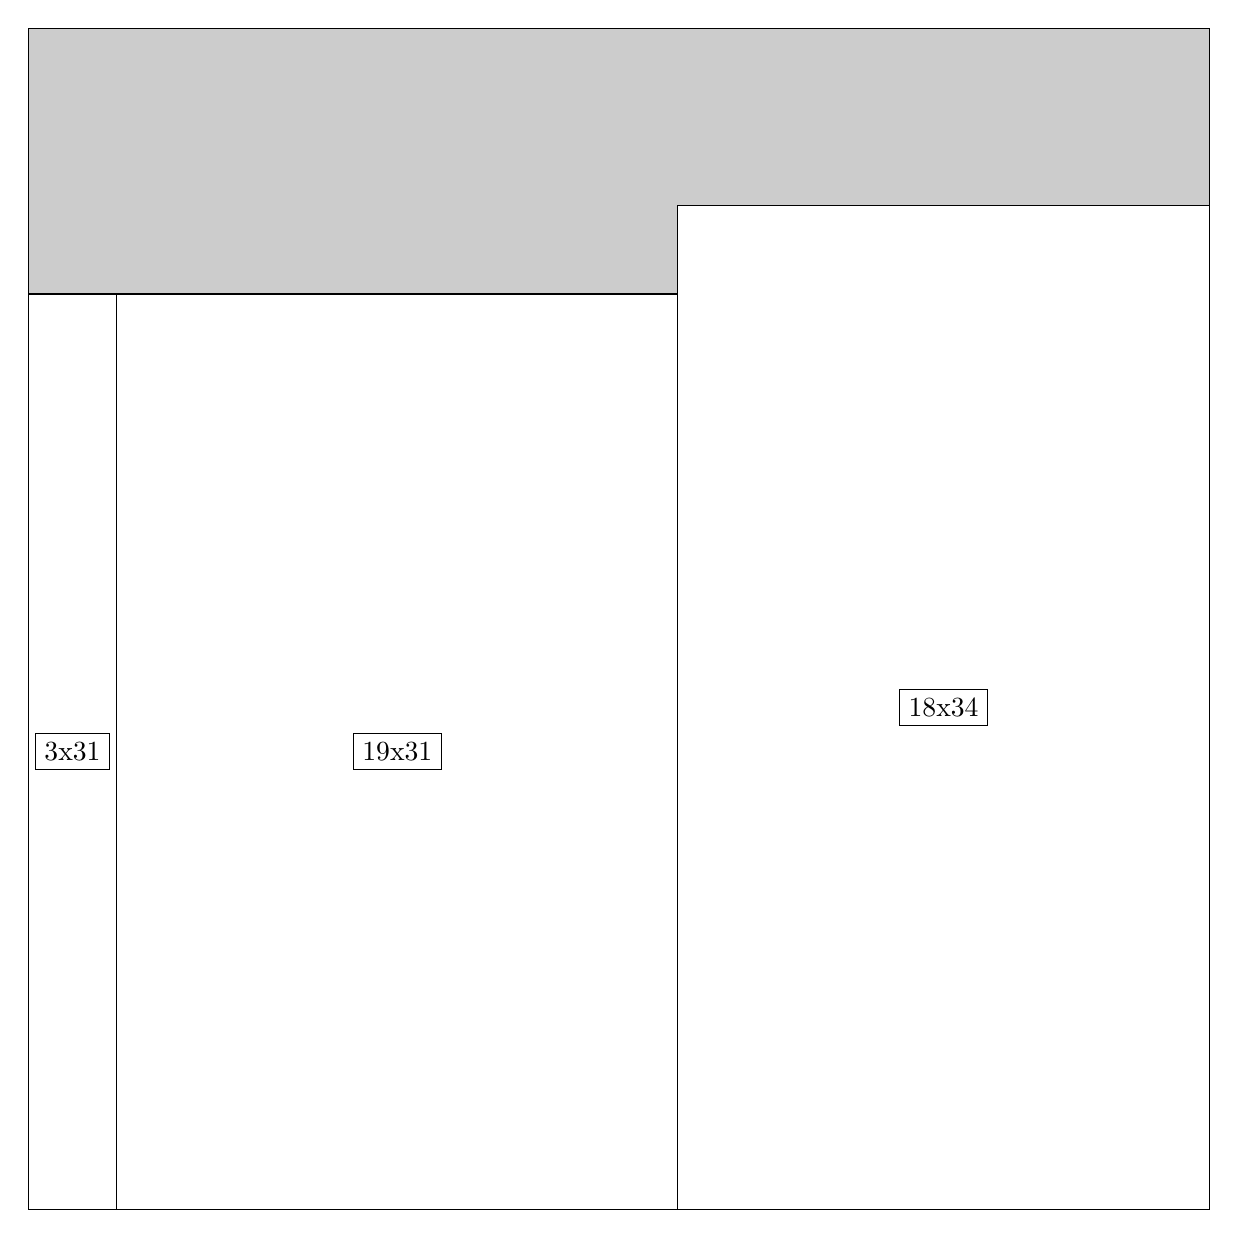
\begin{tikzpicture}[shorten >=1pt,scale=1.0,every node/.style={scale=1.0},->]
\tikzstyle{vertex}=[circle,fill=black!25,minimum size=14pt,inner sep=0pt]
\filldraw[fill=gray!40!white, draw=black] (0,0) rectangle (15.0,15.0);
\foreach \name/\x/\y/\w/\h in {18x34/8.25/0.0/6.75/12.75,19x31/1.125/0.0/7.125/11.625,3x31/0.0/0.0/1.125/11.625}
\filldraw[fill=white!40!white, draw=black] (\x,\y) rectangle node[draw] (\name) {\name} ++(\w,\h);
\end{tikzpicture}


w =18 , h =34 , x =22 , y =0 , v =612
\par
w =19 , h =31 , x =3 , y =0 , v =589
\par
w =3 , h =31 , x =0 , y =0 , v =93
\par
\newpage


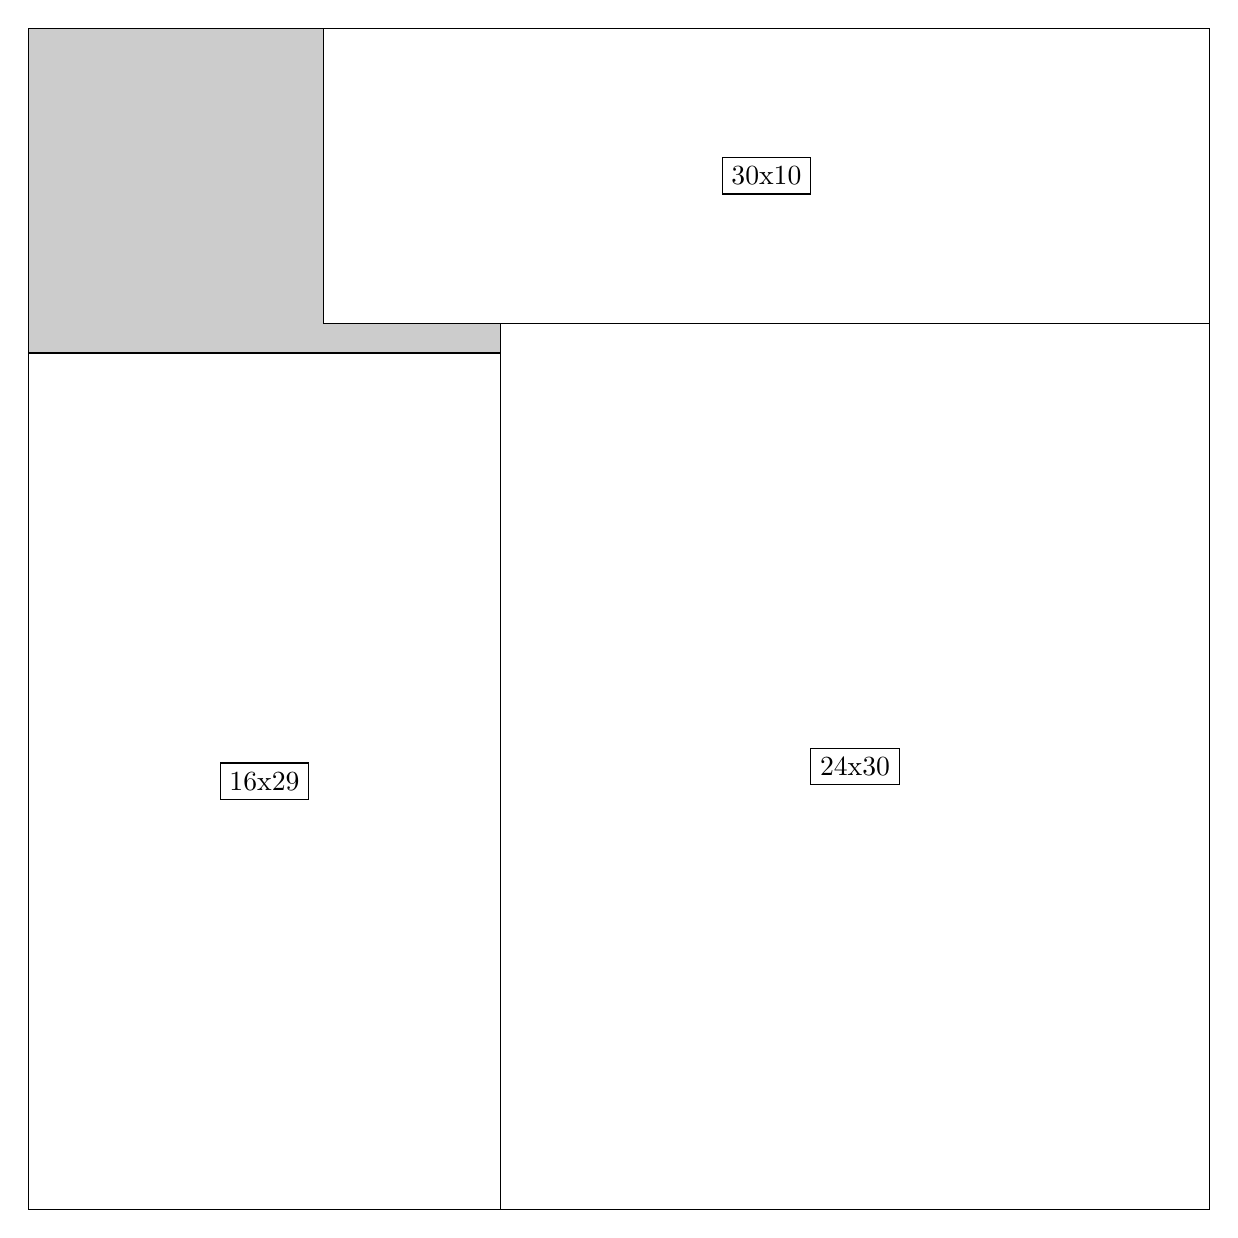
\begin{tikzpicture}[shorten >=1pt,scale=1.0,every node/.style={scale=1.0},->]
\tikzstyle{vertex}=[circle,fill=black!25,minimum size=14pt,inner sep=0pt]
\filldraw[fill=gray!40!white, draw=black] (0,0) rectangle (15.0,15.0);
\foreach \name/\x/\y/\w/\h in {24x30/6.0/0.0/9.0/11.25,16x29/0.0/0.0/6.0/10.875,30x10/3.75/11.25/11.25/3.75}
\filldraw[fill=white!40!white, draw=black] (\x,\y) rectangle node[draw] (\name) {\name} ++(\w,\h);
\end{tikzpicture}


w =24 , h =30 , x =16 , y =0 , v =720
\par
w =16 , h =29 , x =0 , y =0 , v =464
\par
w =30 , h =10 , x =10 , y =30 , v =300
\par
\newpage


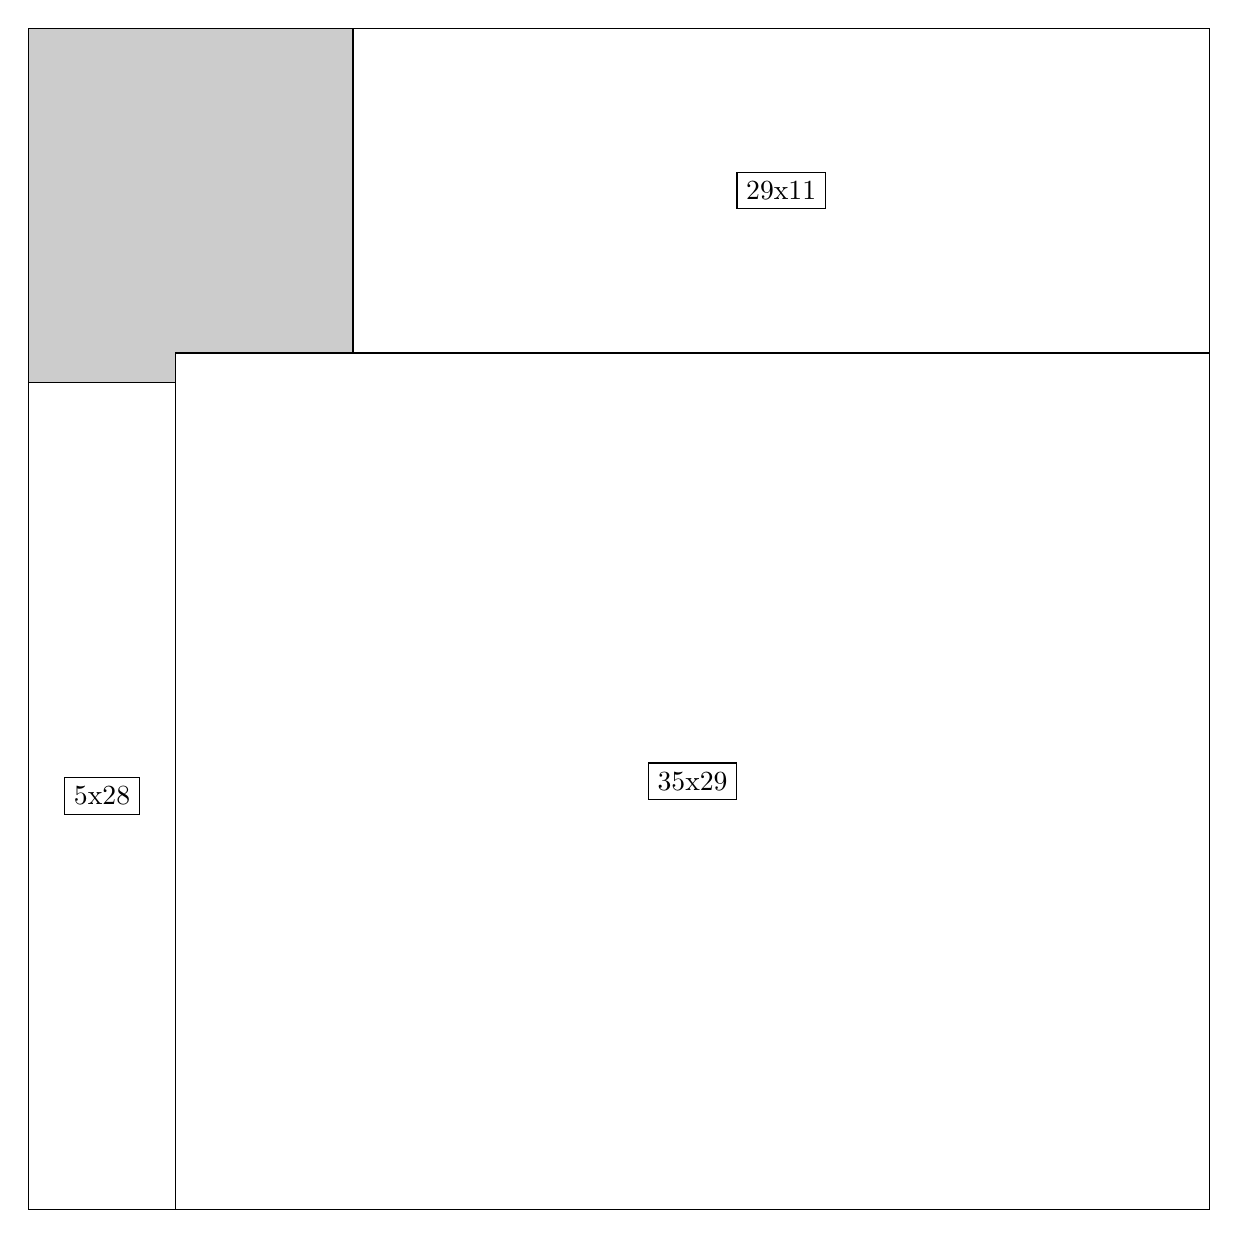
\begin{tikzpicture}[shorten >=1pt,scale=1.0,every node/.style={scale=1.0},->]
\tikzstyle{vertex}=[circle,fill=black!25,minimum size=14pt,inner sep=0pt]
\filldraw[fill=gray!40!white, draw=black] (0,0) rectangle (15.0,15.0);
\foreach \name/\x/\y/\w/\h in {35x29/1.875/0.0/13.125/10.875,5x28/0.0/0.0/1.875/10.5,29x11/4.125/10.875/10.875/4.125}
\filldraw[fill=white!40!white, draw=black] (\x,\y) rectangle node[draw] (\name) {\name} ++(\w,\h);
\end{tikzpicture}


w =35 , h =29 , x =5 , y =0 , v =1015
\par
w =5 , h =28 , x =0 , y =0 , v =140
\par
w =29 , h =11 , x =11 , y =29 , v =319
\par
\newpage


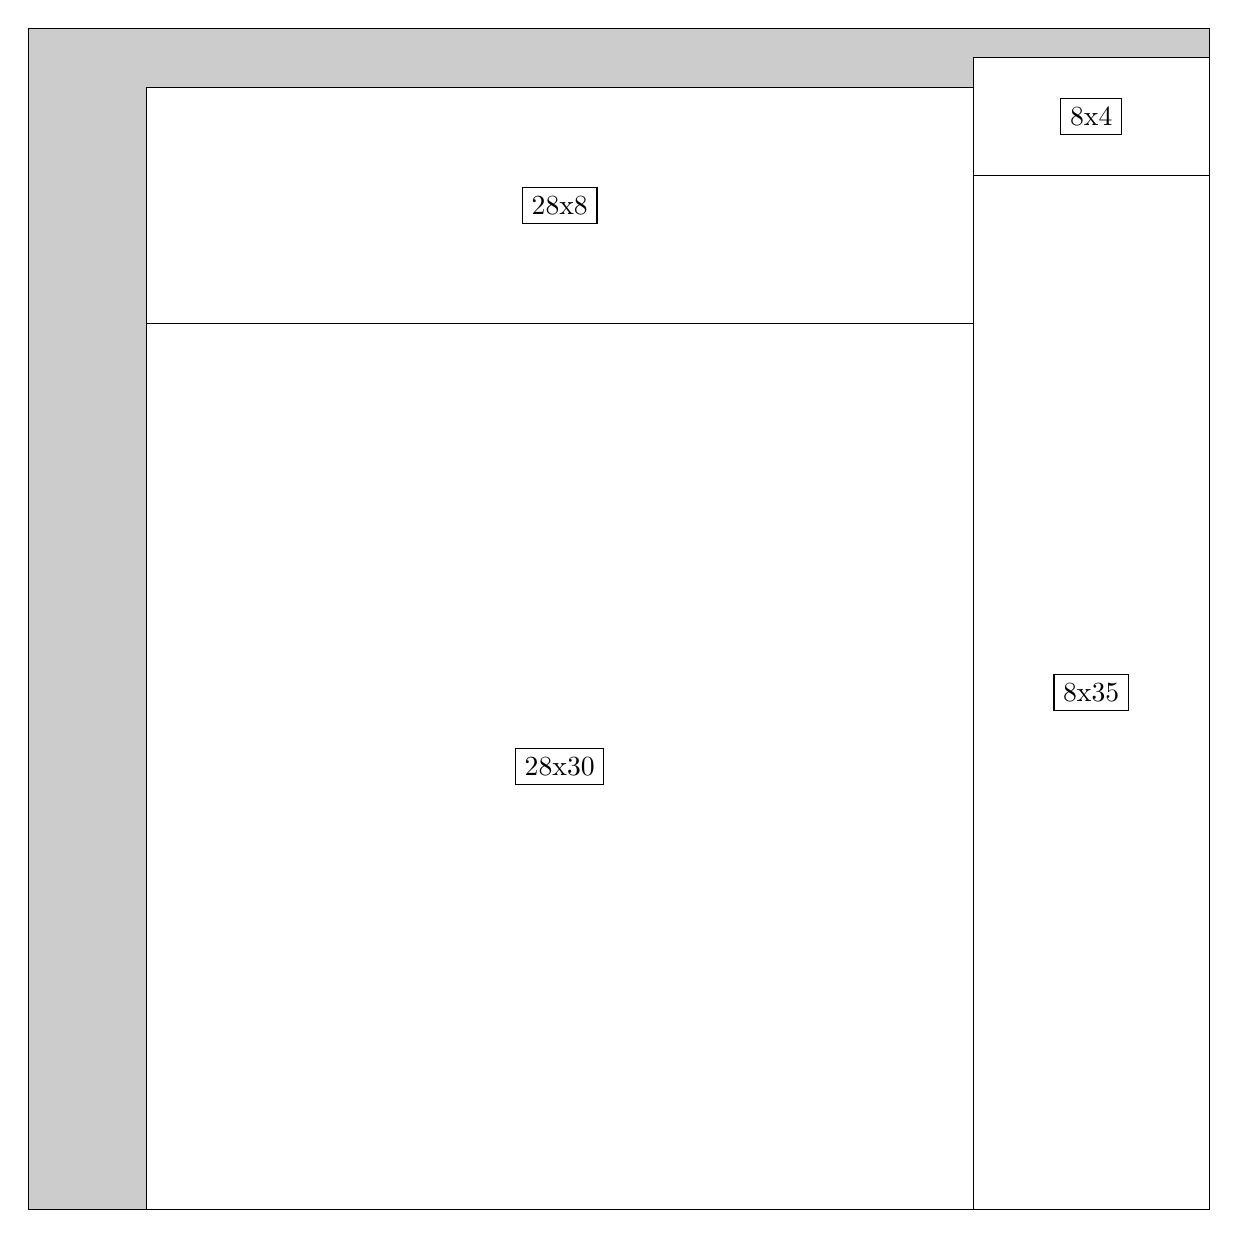
\begin{tikzpicture}[shorten >=1pt,scale=1.0,every node/.style={scale=1.0},->]
\tikzstyle{vertex}=[circle,fill=black!25,minimum size=14pt,inner sep=0pt]
\filldraw[fill=gray!40!white, draw=black] (0,0) rectangle (15.0,15.0);
\foreach \name/\x/\y/\w/\h in {8x35/12.0/0.0/3.0/13.125,8x4/12.0/13.125/3.0/1.5,28x30/1.5/0.0/10.5/11.25,28x8/1.5/11.25/10.5/3.0}
\filldraw[fill=white!40!white, draw=black] (\x,\y) rectangle node[draw] (\name) {\name} ++(\w,\h);
\end{tikzpicture}


w =8 , h =35 , x =32 , y =0 , v =280
\par
w =8 , h =4 , x =32 , y =35 , v =32
\par
w =28 , h =30 , x =4 , y =0 , v =840
\par
w =28 , h =8 , x =4 , y =30 , v =224
\par
\newpage


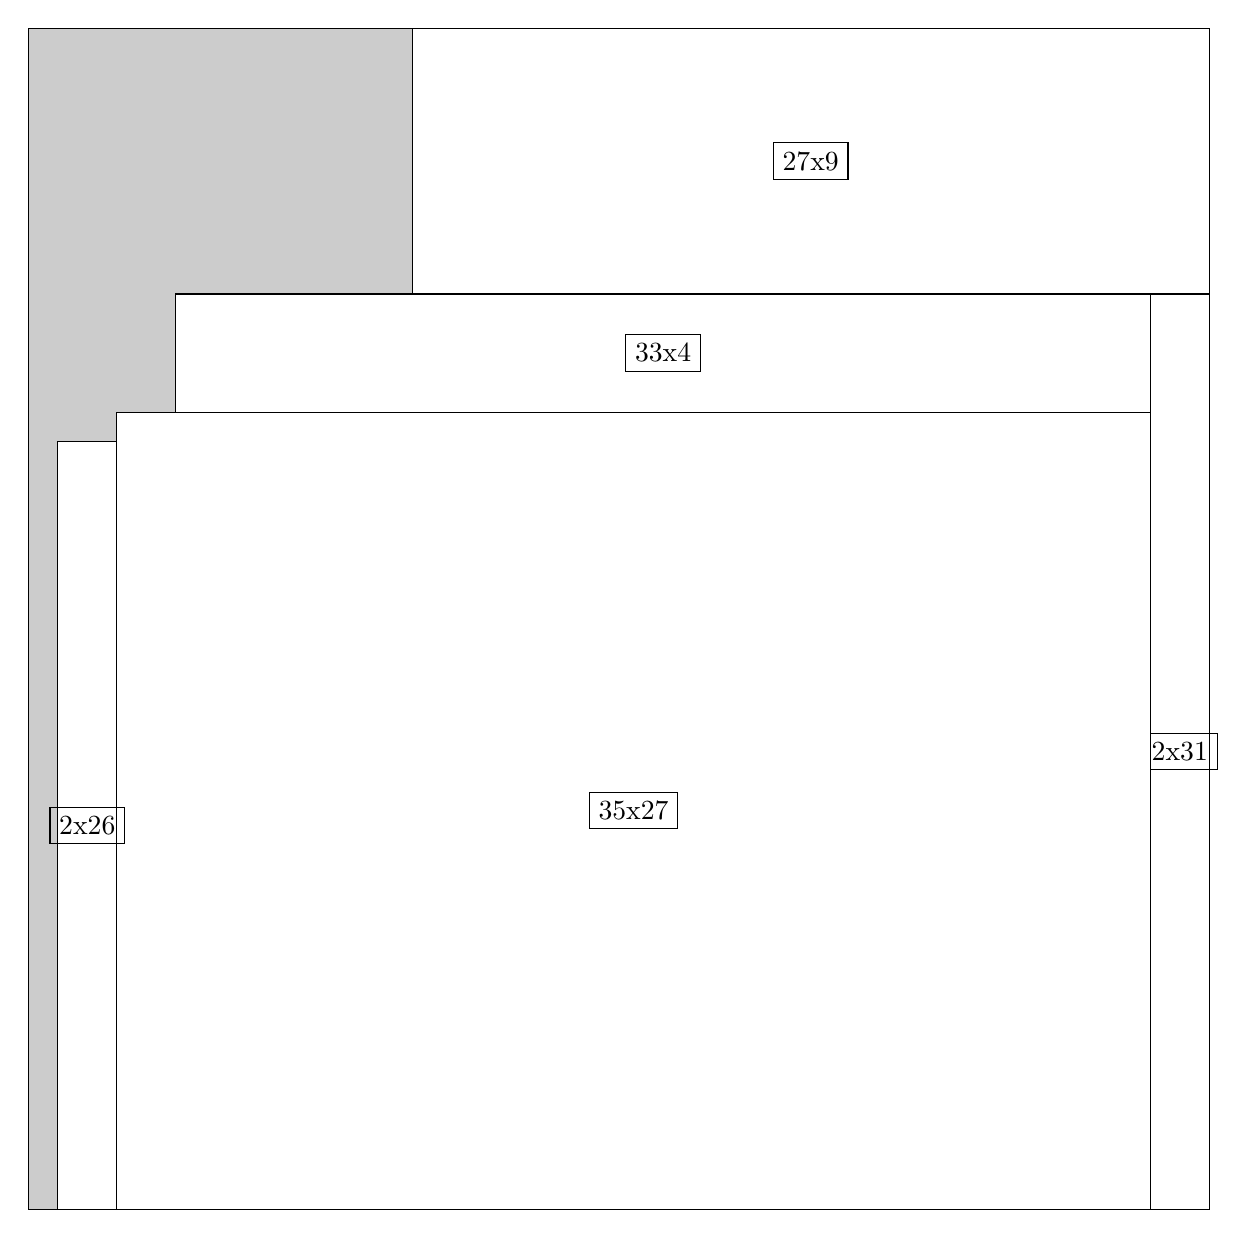
\begin{tikzpicture}[shorten >=1pt,scale=1.0,every node/.style={scale=1.0},->]
\tikzstyle{vertex}=[circle,fill=black!25,minimum size=14pt,inner sep=0pt]
\filldraw[fill=gray!40!white, draw=black] (0,0) rectangle (15.0,15.0);
\foreach \name/\x/\y/\w/\h in {2x31/14.25/0.0/0.75/11.625,35x27/1.125/0.0/13.125/10.125,33x4/1.875/10.125/12.375/1.5,2x26/0.375/0.0/0.75/9.75,27x9/4.875/11.625/10.125/3.375}
\filldraw[fill=white!40!white, draw=black] (\x,\y) rectangle node[draw] (\name) {\name} ++(\w,\h);
\end{tikzpicture}


w =2 , h =31 , x =38 , y =0 , v =62
\par
w =35 , h =27 , x =3 , y =0 , v =945
\par
w =33 , h =4 , x =5 , y =27 , v =132
\par
w =2 , h =26 , x =1 , y =0 , v =52
\par
w =27 , h =9 , x =13 , y =31 , v =243
\par
\newpage


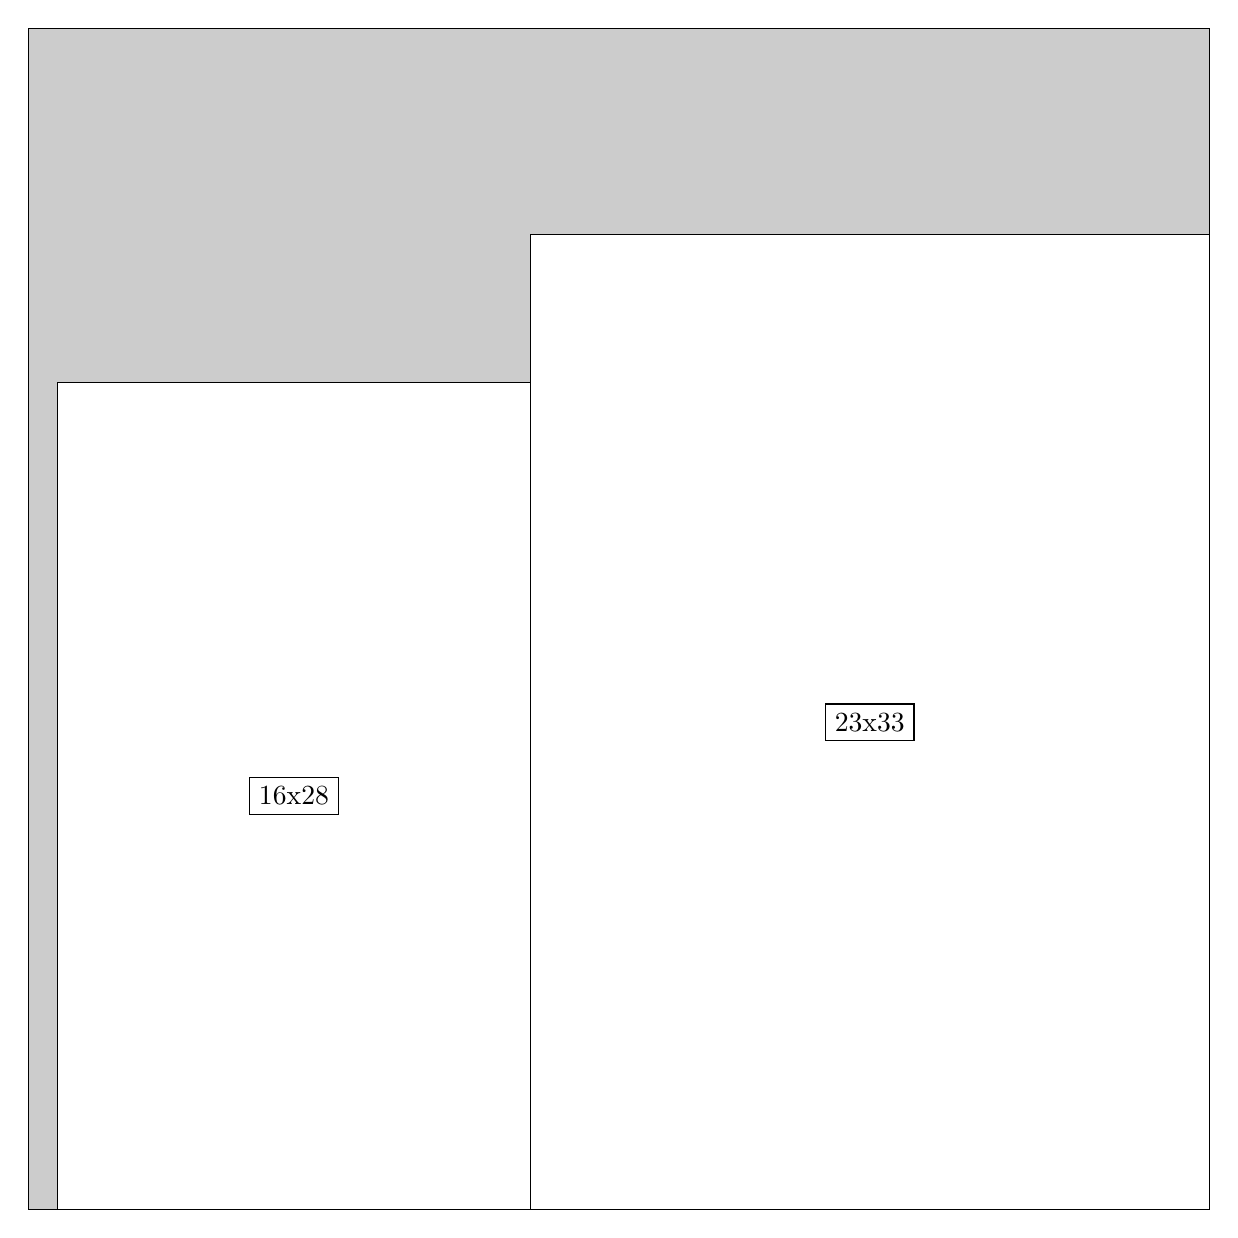
\begin{tikzpicture}[shorten >=1pt,scale=1.0,every node/.style={scale=1.0},->]
\tikzstyle{vertex}=[circle,fill=black!25,minimum size=14pt,inner sep=0pt]
\filldraw[fill=gray!40!white, draw=black] (0,0) rectangle (15.0,15.0);
\foreach \name/\x/\y/\w/\h in {23x33/6.375/0.0/8.625/12.375,16x28/0.375/0.0/6.0/10.5}
\filldraw[fill=white!40!white, draw=black] (\x,\y) rectangle node[draw] (\name) {\name} ++(\w,\h);
\end{tikzpicture}


w =23 , h =33 , x =17 , y =0 , v =759
\par
w =16 , h =28 , x =1 , y =0 , v =448
\par
\newpage


\end{document}